\section{Introduction}
\label{sec:intro}
\begin{figure}
    \centering
    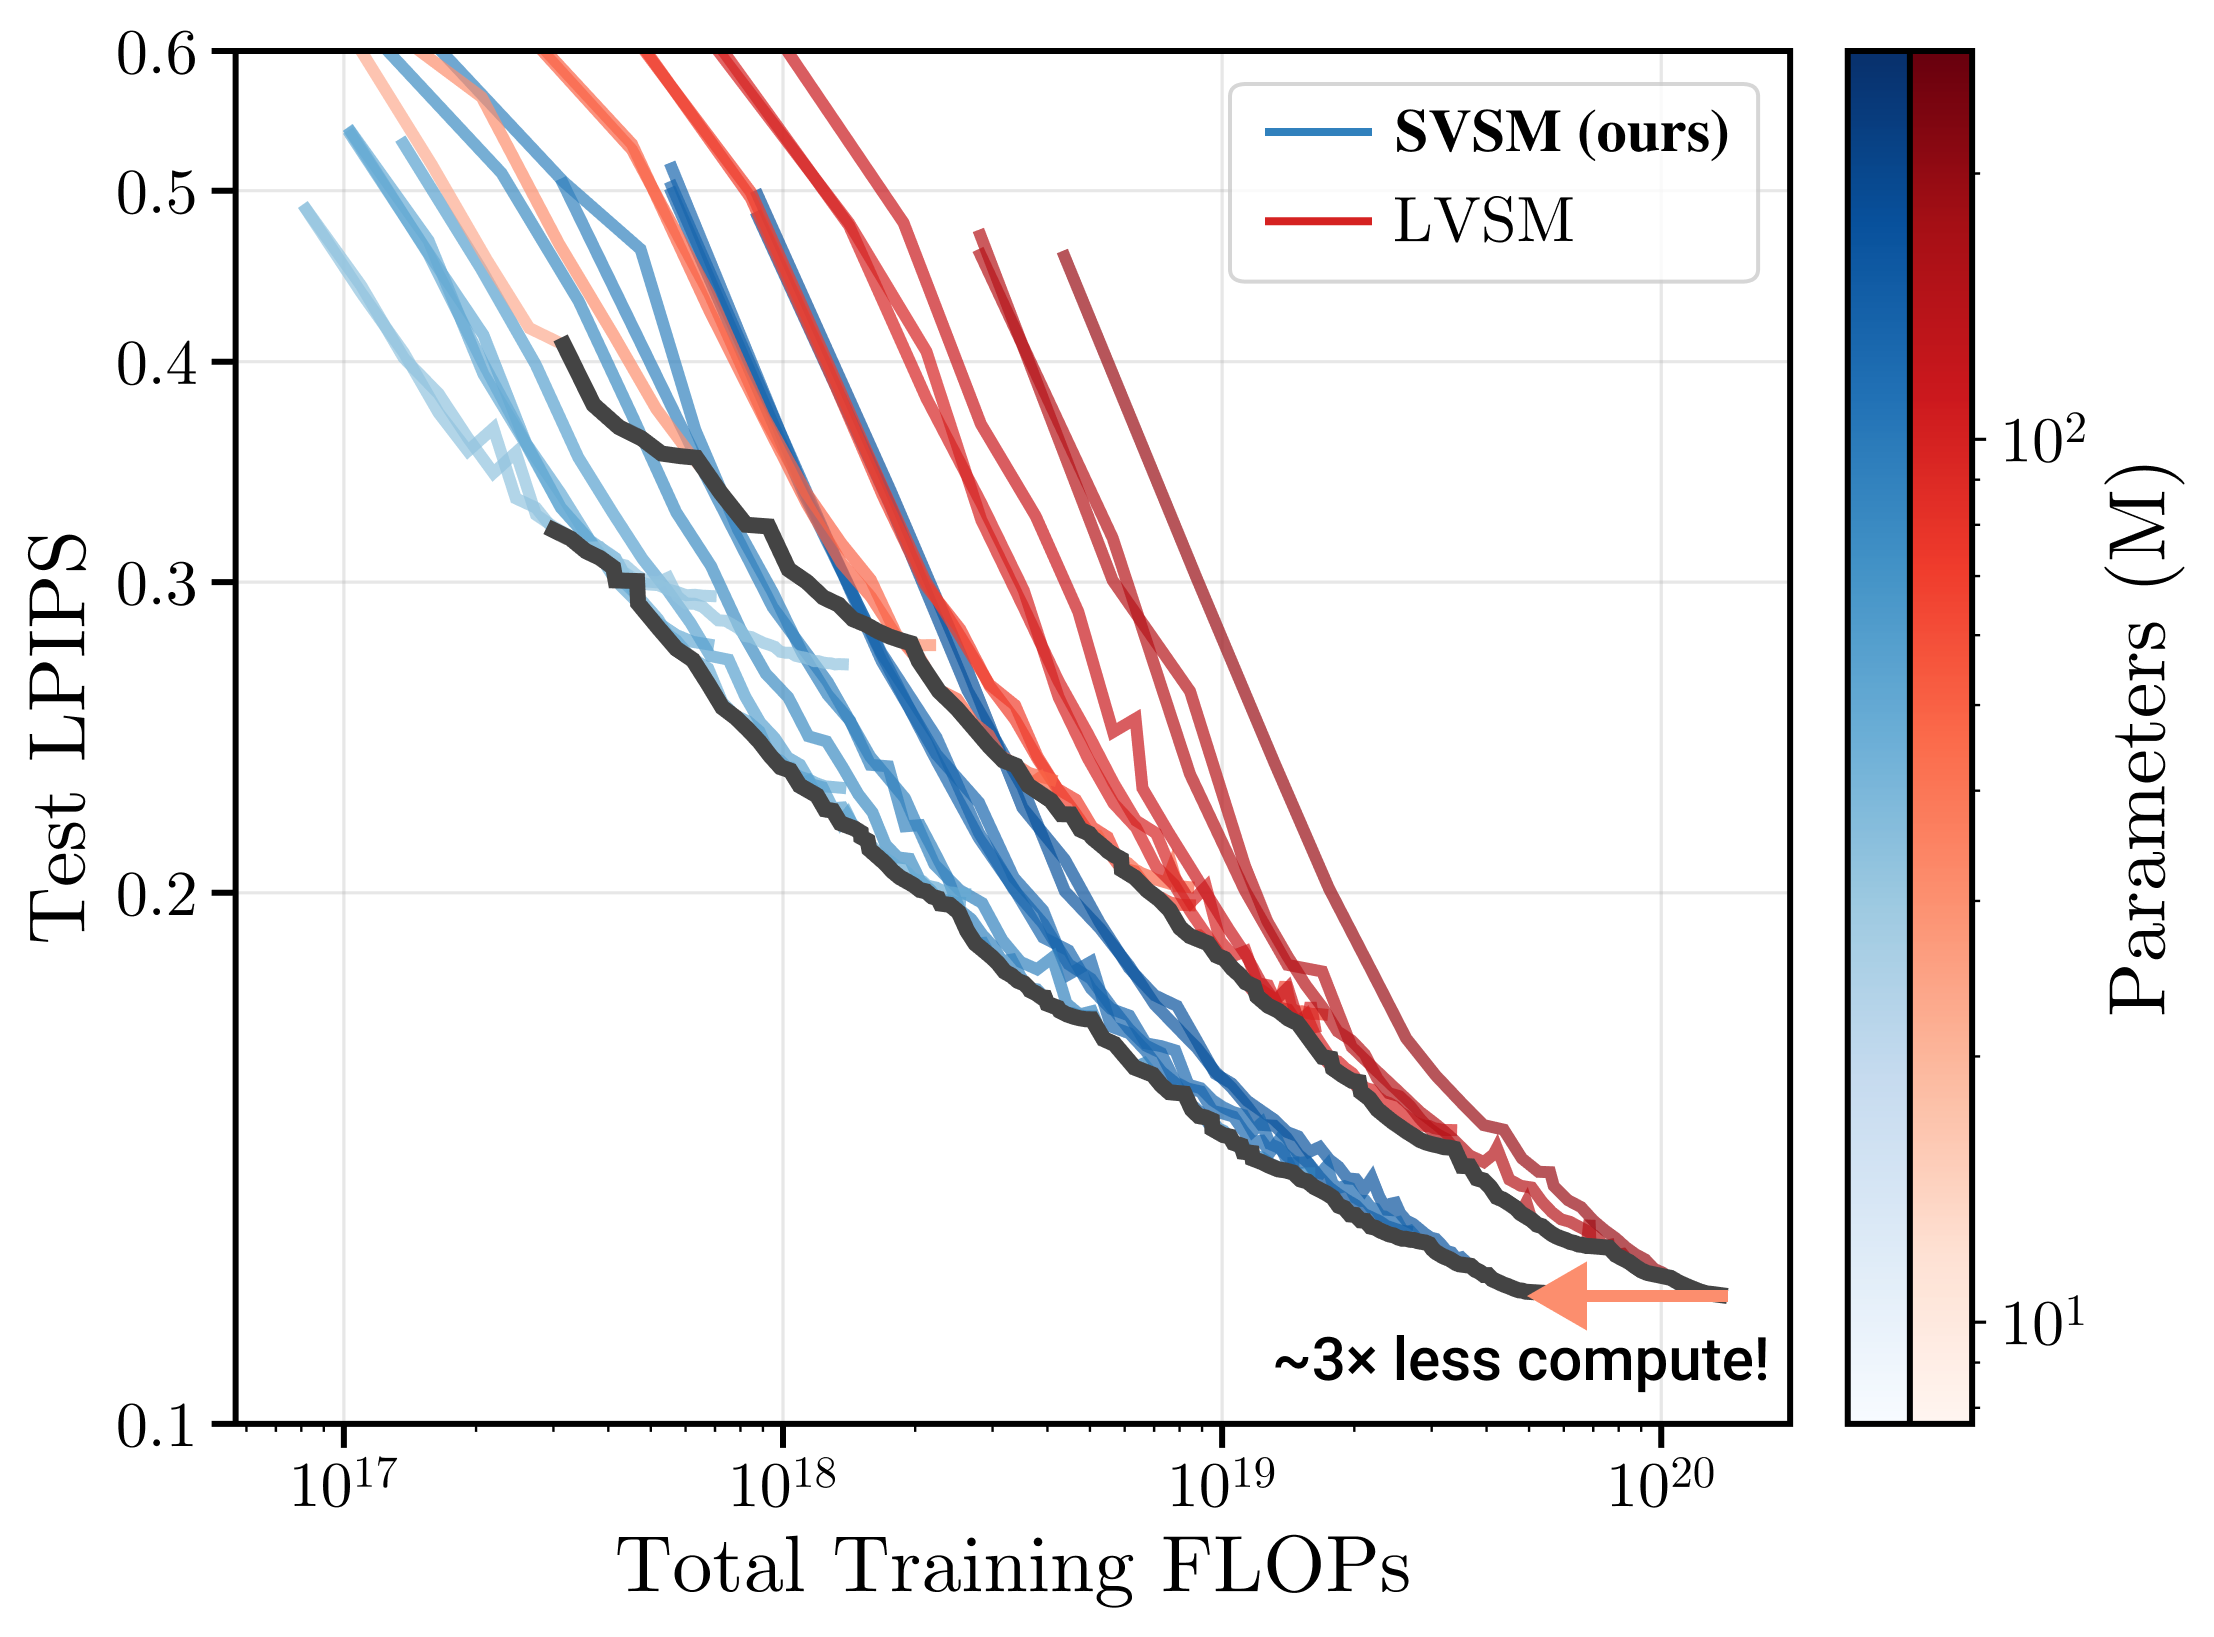
\includegraphics[width=0.9\linewidth]{images/teaser_flop_fixed_final.png}
    \caption{
    % \textbf{Scaling Laws for View Synthesis Transformers.} Evaluated on RealEstate10K~\citep{zhou2018stereo}, SVSM exhibits a more compute-optimal Pareto frontier than LVSM while retaining the same scaling behavior (similar slope and curvature everywhere) while requiring roughly $3\times$ less compute. Though neither frontier is strictly linear, it is clear that both will continue to scale similarly with more compute.
    \textbf{Scaling Laws for View Synthesis Transformers.} Evaluated on RealEstate10K~\citep{zhou2018stereo}, our SVSM exhibits a $3\times$ more compute-optimal Pareto frontier than LVSM while retaining the same scaling behavior (similar slope and curvature everywhere). 
    % Though neither frontier is strictly linear, it is clear that both will continue to scale similarly with more compute.
    % \vspace{-1\baselineskip}
    }
    \label{fig:two-view-scale}
\end{figure}

%
Given a set of images of a scene with known camera poses, the goal of Novel View Synthesis (NVS) is to render novel views of the scene from arbitrary viewpoints. Single scene approaches such as NeRF~\citep{mildenhall2021nerf} and Gaussian Splatting~\citep{kerbl20233d} have achieved impressive fidelity by explicitly modeling 3D geometry and rendering. 
%
Feed-forward extensions of these frameworks train neural networks to reconstruct the 3D representation, achieving promising results~\citep{yu2020pixelnerf,charatan2024pixelsplat,chen2024mvsplat,zhang2024gs}.  However, their formulation inherits handcrafted 3D structure, constraining their ability to scale and handle more complex artifacts such as reflections or transparency.

% Neural networks can be trained to perform this task in a feed-forward manner across diverse scenes, an approach known as generalizable novel view synthesis. Inspired by the success of overfitting-based methods~\cite{}, one line of work employs handcrafted geometric components, such as differentiable renderers, in the model architecture. However, such explicit 3D structure is not necessary for view synthesis: Indeed, recent state-of-the-art approaches [9, 10, 17] have achieved superior results by foregoing geometric inductive biases entirely in favor of pure end-to-end transformer architectures that learn to synthesize views directly as the output of the neural net..
% Over the last decade, Novel View Synthesis (NVS) has emerged as a canonical task in computer vision. 

Typified by Large View Synthesis Model (LVSM)~\cite{jin2024lvsm}, a new class of view synthesis models have emerged which achieve state-of-the-art rendering quality using pure transformer architectures with fewer (if any) geometric inductive biases~\cite{jin2024lvsm, jiang2025rayzer, mitchel2025true, sajjadi2022scene}. However, this class of models is relatively new, and their design space remains unexplored. In particular, training a NVS model involves making design choices over a large number of variables, including the number of context and target views, camera pose parameterizations, attention mechanisms, etc., and there does not yet exist a rigorous investigation of how these choices affect the performance, training efficiency, and inference throughput. To this point, while there exist extensive scaling analyses in language modeling and 2D vision~\cite{esser2024scaling, hoffmann2022training, kaplan2020scaling, peebles2023scalable, zhai2022scaling}, there exists no analogue for 3D vision. Thus, the goal of this work is to provide such an analysis in addition to a compute-optimal training recipe for view synthesis transformers in terms of both architecture and training strategy.


In particular, we first challenge the necessity of the decoder-only architecture proposed in LVSM~\citep{jin2024lvsm}. While powerful, it requires passing all context images through the entire transformer each time a \textit{single} target image is decoded. It is a \emph{bidirectional} model where both the target view tokens \emph{and} context view tokens are updated in each layer of the network. While this allows the model to consider only information in the context images that is relevant to the target view, it incurs substantial computational cost due to repeated processing of context views.

Instead, we advocate for an encoder-decoder design which produces an intermediate scene latent representation. This approach is potentially far more efficient: the computational cost of constructing the scene representation is amortized through repeated calls to the decoder, which efficiently extracts information from the representation via \emph{unidirectional} cross attention from scene to target.  However, the scene representation also represents an information bottleneck. Without a proper training strategy that maximally leverages the efficiency of the encoder-decoder design, it can be challenging for encoder-decoder models to outperform decoder-only models. Here, we identify that the key for unlocking the potential of encoder-decoder models lies in the way target views (\emph{i.e.} the reconstruction targets) are utilized during training. The implicit standard practice employed by prior work~\citep{charatan2024pixelsplat, jin2024lvsm, sajjadi2022scene, zhang2024gs} has been to reconstruct multiple different target views from a single scene during training. However, the consequences of this approach have never been fully analyzed. To this point, we propose and empirically validate the \emph{effective batch hypothesis}, which argues that reconstructing multiple target views per scene effectively multiplies the batch size.  

%As a result, shared information across multiple views cannot be preprocessed in an amortized manner and instead must be recomputed each time a new target image is rendered, making both the training and inference largely inefficient. 
%There is no precomputed encoding of the scene, which is in contrast to traditional 3D pipelines in which efficient rendering is possible from a prebuilt 3D scene representation.


% However, involving a scene representation inevitably introduces a significant bottleneck. By definition, a scene encoder cannot expect specific target view in advance. A valid scene representation must be decodable from any viewpoints within reasonable range. On the other hand, a decoder-only model can proactively focus its resource on processing information that is only relevant to the target view. 
% As a result, there is a nontrivial trade-off 


% There is no precomputed encoding of the scene, and each view must be computed from the raw images themselves, 
% This is in contrast to traditional 3D vision pipeline where efficient rendering is possible from ...3D...
%  We find that an encoder combined with a cross-attention based decoder alleviates this issue by allowing for parallel decodes of multiple target images. 
% , models can use more parameters for the same amount of compute, allowing for better flop-matched performance.


% Secondly, we elucidate the meaning of target views in training. The standard in training feed-forward NVS models has been to use several target views~\citep{charatan2024pixelsplat, jin2024lvsm, sajjadi2022scene, zhang2024gs} for supervision per scene, but it is unclear what the purpose of this is. Through several experiments, we find that it effectively acts as a multiplier on the batch size. This points to the benefit of efficient decoding of multiple targets -- it raises your batch size for a sublinear increase in FLOPs [maybe remove and explain in body].




% , maximizing the training throughput. By a thorough investigation, we confirm this hypothesis.
% By a thorough investigation, we confirm that this practice of using multiple target views effectively acts as a multiplier on the batch size, thereby maximizing the training throughput.
% propose and confirm the 

% Through several experiments, we find that it effectively acts as a multiplier on the batch size. This points to the benefit of efficient decoding of multiple targets -- it raises your batch size for a sublinear increase in FLOPs [maybe remove and explain in body].

% it is highly inefficient... Following the wisdom of LLM researches, we argue that the same scalability is achievable without inefficient bidirectional update...

% Lastly, we find that the recently proposed relative camera pose embedding~\citep{li2025cameras} is critical for many-view settings, when more context has to be processed. 

% We test these architectural changes across approximately 3 orders of magnitude of training compute, which we find is enough to show consistent scaling trends. 

These insights yield a principled transformer view synthesis model, which we call the \textit{Scalable View Synthesis Model} (SVSM), that fully capitalizes on the rendering efficiency of a unidirectional encoder-decoder architecture, maximizing training throughput without compromising performance or scalability.
We demonstrate that our unidirectional model scales as efficiently as bidirectional models, which aligns with the scalability of causal, unidirectional attention in large language models~\citep{kaplan2020scaling}. 
As part of this analysis, we also reveal scaling relationships within view synthesis that parallel those observed in the Chinchilla language model family~\citep{hoffmann2022training}.
Finally, we demonstrate that SVSM achieves state-of-the-art results in real-world NVS tasks with significantly reduced compute, challenging the previous understanding that bidirectional attention is critical to high-fidelity view synthesis~\citep{jin2024lvsm}.

% As a result of this analysis, we recover data-model scaling relationships within the NVS domain that closely parallel those observed in the Chinchilla scaling laws~\citep{hoffmann2022training}.
\vspace{-0.5\baselineskip}
\paragraph{Key Contributions:}
\begin{itemize}
    \item We provide the first rigorous scaling analysis for novel view synthesis transformers.
    \item We propose and empirically confirm the \textit{effective batch size hypothesis} that unlocks compute-optimal training.
    \item We show that bidirectional decoding is not critical for scalable view synthesis, contrasting recent work~\cite{jin2024lvsm}.
    \item Based on this analysis, we present a compute-optimal model that achieves a new state-of-the-art in real-world NVS tasks with substantially reduced training compute. 
\end{itemize}



% ... Removing these strong assumptions enable state-of-the-art recon quality... 



% By leveraging these findings, we provide the compute-optimal strategy for NVS model... This is the first work to discuss the scaling law of NVS models with rigor... we elucidate the several novel scaling factors specific to NVS problems...

% \noindent \textbf{Our core contributions are summmarized as follows:}




